\section{System architecture}
\label{sec:systemarchitecture}
\subsection{Overview}

The implemented runtime is a LangGraph directed acyclic graph with five specialised agents and a shared typed state object. Its default configuration names \texttt{openai/gpt-oss-20b} for text and \texttt{qwen/qwen3.8-27b} for vision through Groq. The backtest path enforces point-in-time input windows, shared upstream reports for paired variants, structured binary decisions, and a separate compounded-account ledger.

\subsection{Indicator Agent}
The Indicator Agent computes five momentum and volatility oscillators using TA-Lib over the most recent OHLCV window, including MACD \cite{appel2005technical}, RSI \cite{wilder1978new}, Stochastic Oscillator \cite{lane1984stochastic}, Williams \%R \cite{williams1973trading}, and ROC-based momentum signals \cite{murphy1999technical}. Table~\ref{tab:indicator_conditions} lists each indicator with its parameters and signal classification rules. Signal classification is performed deterministically in Python before any LLM call, using hard thresholds and two-bar crossover detection. The classified counts-number of bullish, bearish, and neutral signals-are injected directly into the LLM prompt as immutable ground-truth constraints, preventing the model from hallucinating signal tallies. A majority rule then determines an overall consensus with an associated confidence level (High if four or more signals agree, Medium if three agree, Low otherwise).

\begin{table}[H]
\centering
\caption{Technical indicators and trading signal conditions}
\label{tab:indicator_conditions}
\renewcommand{\arraystretch}{1.2}

\begin{tabularx}{\textwidth}{|l|l|X|X|}
\hline
\textbf{Indicator} & \textbf{Parameters} & \textbf{Bullish condition} & \textbf{Bearish condition} \\
\hline

MACD & 12, 26, 9 &
Golden cross or positive histogram expanding &
Death cross or negative histogram expanding \\
\hline

RSI & period = 14 &
$\leq 30$ (oversold) or value $\geq 55$ &
$\geq 70$ (overbought) or value $\leq 45$ \\
\hline

Stochastic & 14, 3, 3 &
\%K crosses above \%D, or \%K $\leq 20$ &
\%K crosses below \%D, or \%K $\geq 80$ \\
\hline

Williams \%R & period = 14 &
\%R $\leq -80$ or trending toward 0 &
\%R $\geq -20$ or trending toward $-100$ \\
\hline

ROC & period = 10 &
ROC $> +0.5\%$ &
ROC $< -0.5\%$ \\
\hline

\end{tabularx}
\end{table}

\subsection{Alpha Agent}

The Alpha Agent serves two explicitly separated functions: OHLCV-only quantitative factor evaluation and qualitative comparison with Vietnamese sentiment supplied as textual LLM context.

\paragraph{Alpha selection.}
An offline registry of 85 candidate alpha functions is maintained, comprising five proprietary single-stock momentum and reversion formulas (Table~\ref{tab:proprietary_alphas}) and 80 adaptations of the WorldQuant 101 Formulaic Alphas to single-stock OHLCV data. Cross-sectional operators such as \texttt{ts\_rank} are adapted to their single-asset time-series analogues (i.e., rolling percentile rank over the lookback window). We acknowledge that this translation alters the statistical properties of the original factors: without the cross-sectional dispersion that drives many WQ-101 alphas, single-asset surrogates may exhibit faster signal decay, higher autocorrelation, and reduced distributional stability. A full per-factor diagnostic examining IC decay profiles, signal autocorrelation, and factor turnover rates is left to future work (see Section~\ref{sec:limitations_futurework}). When the volume series is unavailable or sparse, intra-bar price range is used as a proxy.

For a given symbol and timeframe, the available point-in-time history is truncated to at most 600 bars ending at the decision cutoff. Features (returns, log-volume, VWAP proxy, and ADV20) are then constructed. Candidate metrics use only matured net Open-to-Close labels within this snapshot; the final $L$ rows are excluded because their targets are unavailable at the cutoff. A zero net return is assigned \texttt{DOWN}, consistent with the requirement that a LONG must remain profitable after costs.

The selector computes Spearman Information Coefficient (IC), directional accuracy on signals above the configured absolute threshold, and a horizon Sharpe diagnostic. Long-only win rate and other economic summaries are retained for diagnosis but do not enter the composite score.

A candidate is eligible only when it has at least 20 finite observations and finite ranking metrics. Ineligible candidates are removed \emph{before} the per-metric min--max bounds are computed. Using $\mathcal{N}_{\mathcal{V}}$ from Equation~\eqref{eq:candidate_minmax}, the default composite score is:

\begin{equation}
S = 0.40\mathcal{N}_{\mathcal{V}}(|IC|)
  + 0.35\mathcal{N}_{\mathcal{V}}(Acc)
  + 0.25\mathcal{N}_{\mathcal{V}}(Sharpe)
\label{eq:composite_score}
\end{equation}

If a metric is constant across the eligible set, its normalised value is $0.5$ for every candidate. The displayed coefficients are the default runtime weights; robustness configurations replace them with recorded alternatives. Long-only accuracy is excluded from ranking to avoid rewarding a factor solely because the historical sample trends upward.

Up to five eligible candidates are selected for the current prediction. When historical IC is negative, the signal is multiplied by $-1$ for metric computation and current inference. All observations used for this orientation precede the decision cutoff, but estimating orientation and rank on the same finite history can still overfit to noise. Bootstrapped IC confidence intervals or a Deflated Sharpe adjustment~\cite{bailey2014deflated,harvey2016} would provide stronger guarantees of signal stability.

\begin{table}[htb]
\centering
\caption{Five proprietary alpha formulas}
\label{tab:proprietary_alphas}
\renewcommand{\arraystretch}{1.25}

\begin{tabularx}{\textwidth}{|c|l|X|}
\hline
\textbf{Alpha} & \textbf{Name} & \textbf{Formula} \\
\hline

$\alpha_1$ &
Flow-Driven Momentum &
$\tanh(\mathrm{ROC}(1)_{\mathrm{adj}} \times \mathrm{VolSurge} \times 0.5)$ \\
\hline

$\alpha_2$ &
MACD-Flow Proxy &
$\tanh(\mathrm{MACDHist}_{\mathrm{norm}} + \mathrm{ROC}(1)_{\mathrm{adj}} \times 0.5)$ \\
\hline

$\alpha_3$ &
Liquidity Void Reversion &
$\tanh\!\left(-0.8 \times \mathrm{ZScore}\!\left(\frac{\mathrm{Close} - \mathrm{SMA}_5}{\mathrm{Close}}\right)\right)$ \\
\hline

$\alpha_4$ &
Bollinger Squeeze \& Flow &
$\tanh((\%B - 0.5) \times \mathrm{VolZ}_5 \times 1.5)$ \\
\hline

$\alpha_5$ &
Order Flow Exhaustion &
$\tanh(\mathrm{ROC}(1)_{\mathrm{adj}} \times \mathrm{ClosePos} \times 3.0)$ \\
\hline

\end{tabularx}

\vspace{0.5em}

\end{table}


\paragraph{Sentiment integration.}
Articles from CafeF are crawled for the target ticker and up to ten related companies identified by the LLM. The primary scoring path calls the configured \texttt{5CD-AI/}\allowbreak\texttt{Vietnamese-Sentiment-}\allowbreak\texttt{visobert} HF Inference API endpoint; endpoint failure triggers a versioned deterministic lexicon scorer. Every newly scored article stores the actual scorer, requested model identifier, observed Hub revision/status, and fallback status/reason. A run reports the ViSoBERT endpoint identifier only when all included articles verify successful use of that endpoint; mixed, fallback-only, and legacy-unknown runs are labelled accordingly.

Two point-in-time context variables are constructed. $S_{\mathrm{decay}}$ is the exponentially time-weighted mean of all valid dated-and-scored articles in the 90-day window, with a 30-day half-life and strict exclusion of post-cutoff observations. $Rel_{\mathrm{sent}}$ is the difference between the target's time-decayed score and the mean time-decayed score of related companies having at least three valid observations. Either value is marked unavailable when its observation requirement is not met; missing data is not encoded as neutral zero. The full compact observation set is used for these calculations, while the 15-article slice is display-only.

Neither variable is injected into $\alpha_2$, any other registry formula, or factor ranking. They and the per-company related sentiment values are rendered in a separate prompt section that the LLM uses only for qualitative comparison with the OHLCV factor report.

In backtest mode, the live crawler is replaced by a pre-loaded historical sentiment store keyed by symbol and decision timestamp. Inclusion is based on timezone-aware \texttt{available\_at}, not merely a publication date: date-only CafeF records become available at 00:00 on the next day in \texttt{Asia/}\allowbreak\texttt{Ho\_Chi\_Minh}, and undated records are rejected rather than used as fallback.

\begin{figure}[htb]
    \centering
    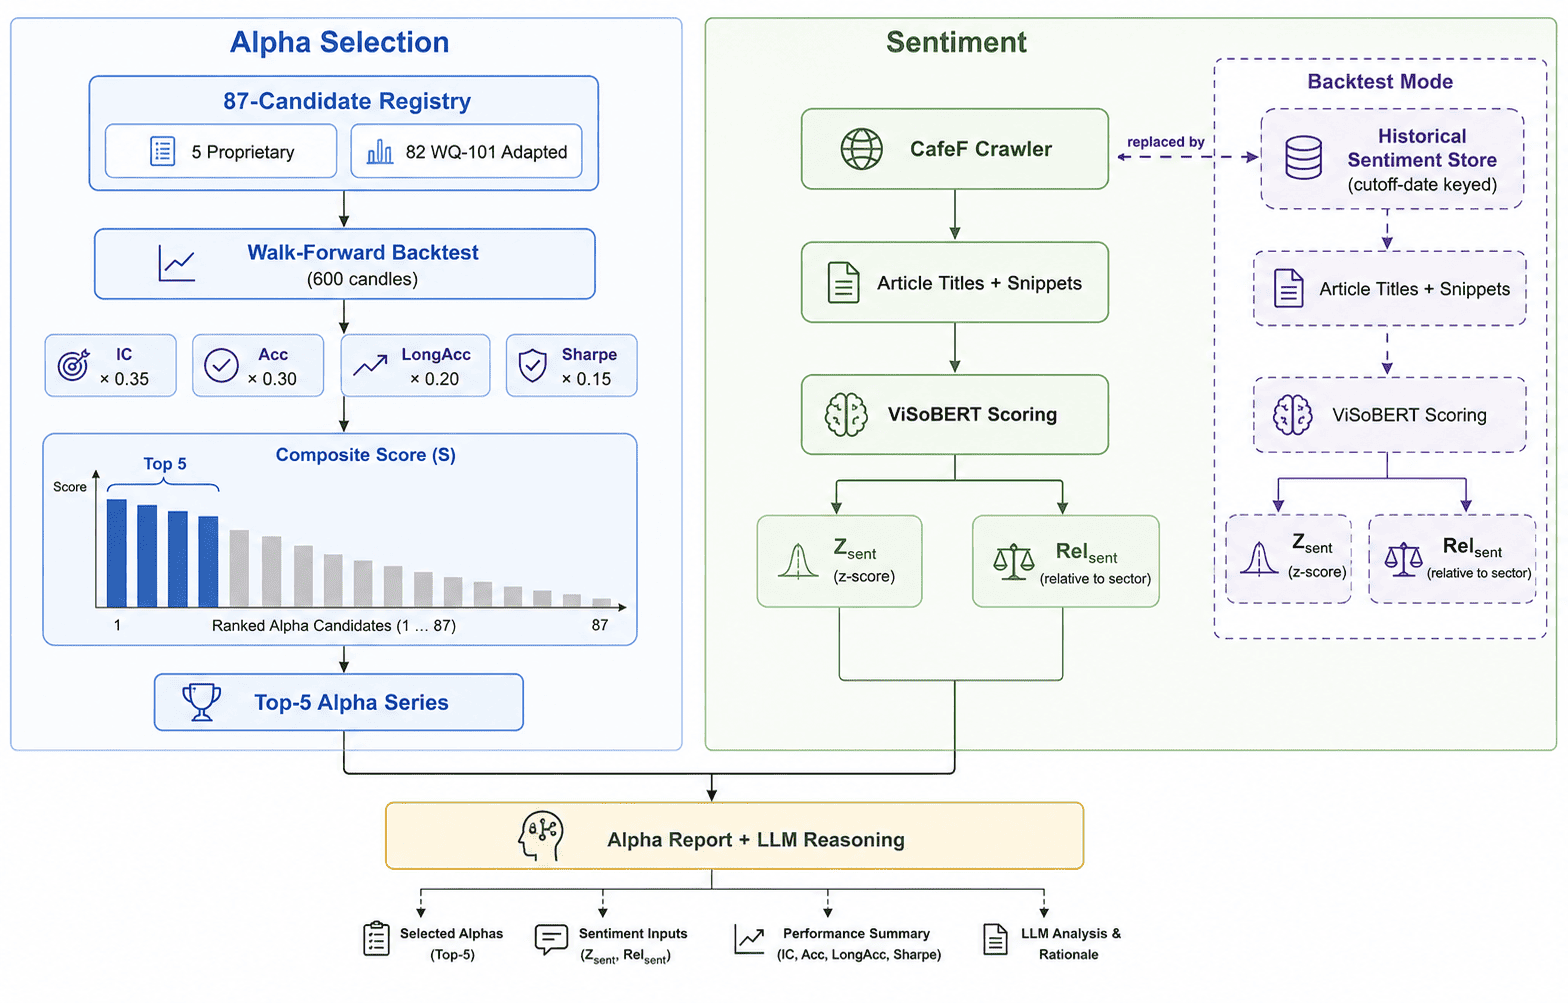
\includegraphics[width=0.9\textwidth]{figs/alpha_agent_pipeline.png}
    \caption{Internal data flow of the Alpha Agent}
    \label{fig:alpha_agent}
\end{figure}

\subsection{Pattern Agent}

The Pattern Agent analyses a candlestick chart rendered from the current
analysis window $[e-W,e)$ (45 candles in the main configuration). The chart is
produced by \texttt{mplfinance} using a custom colour scheme (green bodies for
bearish candles and red bodies for bullish candles, following Vietnamese market
convention) and encoded as a base64 PNG before graph execution.

The vision-language model is prompted to perform four sequential tasks. First, it identifies the dominant chart formation from a curated list of 16 classical patterns, such as head-and-shoulders inverse, double bottom, or various triangles and wedges. Second, it describes the three to five most recent candles in terms of body size, wick length, and relative position. Third, it assesses whether a breakout or breakdown is occurring. Finally, it commits to a directional bias (\texttt{bullish}, \texttt{bearish}, or \texttt{neutral}) alongside a confidence rating of \texttt{High}, \texttt{Medium}, or \texttt{Low}.

The prompt is explicitly structured to discourage non-committal answers and encourage a directional interpretation whenever sufficient evidence is present.

After inference, a deterministic verifier compares the reported bias with the final candlestick body and the direction of the last five closes. An obvious contradiction is appended to the report and downgrades its confidence. If the vision model fails or no chart image is available, the agent falls back to a text-only analysis of raw OHLCV values using the text LLM.


\subsection{Trend Agent}

The Trend Agent receives a separate chart in which support and resistance lines have been fitted algorithmically before LLM invocation.

Two trendline pairs are computed.

\paragraph{Close-price trend channel.}
The first pair is derived from the closing price series alone. A linear regression line is fitted to all 45 candles in $[e-W,e)$, and the upper and lower deviations from this line identify the resistance and support pivots respectively. The slopes are then refined by minimising squared deviations subject to two constraints: the support line must not intersect any closing price from above, and the resistance line must not intersect any closing price from below.

\paragraph{High-low channel.}
The second pair uses the high and low price series to identify the highest and lowest deviation points, producing channel lines that bound the full intra-bar range.

The support lines are drawn in blue, resistance lines in red, and rendered at 600 DPI to preserve legibility when compressed to base64.

The vision-language model is prompted to assess the slope of each support and resistance line, evaluate the distance between the lines (indicating channel width and price compression), determine the position of the most recent candles relative to each boundary, and produce a directional forecast for the applicable prediction horizon. The required JSON output fields encompass the trend direction, numerical support and resistance levels, slope characterisation, and overall confidence.

After inference, a deterministic verifier checks the reported trend against price relative to SMA20, the availability of SMA50, and the recent price slope. Contradictory claims are flagged and their confidence is reduced. If the vision-language model fails or no rendered chart is available, the agent falls back to a text-only analysis of raw OHLCV data, mirroring the strategy used by the Pattern Agent.


\subsection{Decision Agent}

The Decision Agent synthesises all upstream reports into a single trading judgment. To remain within the Groq token-per-minute limit, each report is condensed before being passed to the prompt: the Indicator report is trimmed to its consensus summary block, the Alpha report retains only the factor table and LLM reasoning paragraph, and the Sentiment report drops the per-article listing.

\begin{figure}[htb]
    \centering
    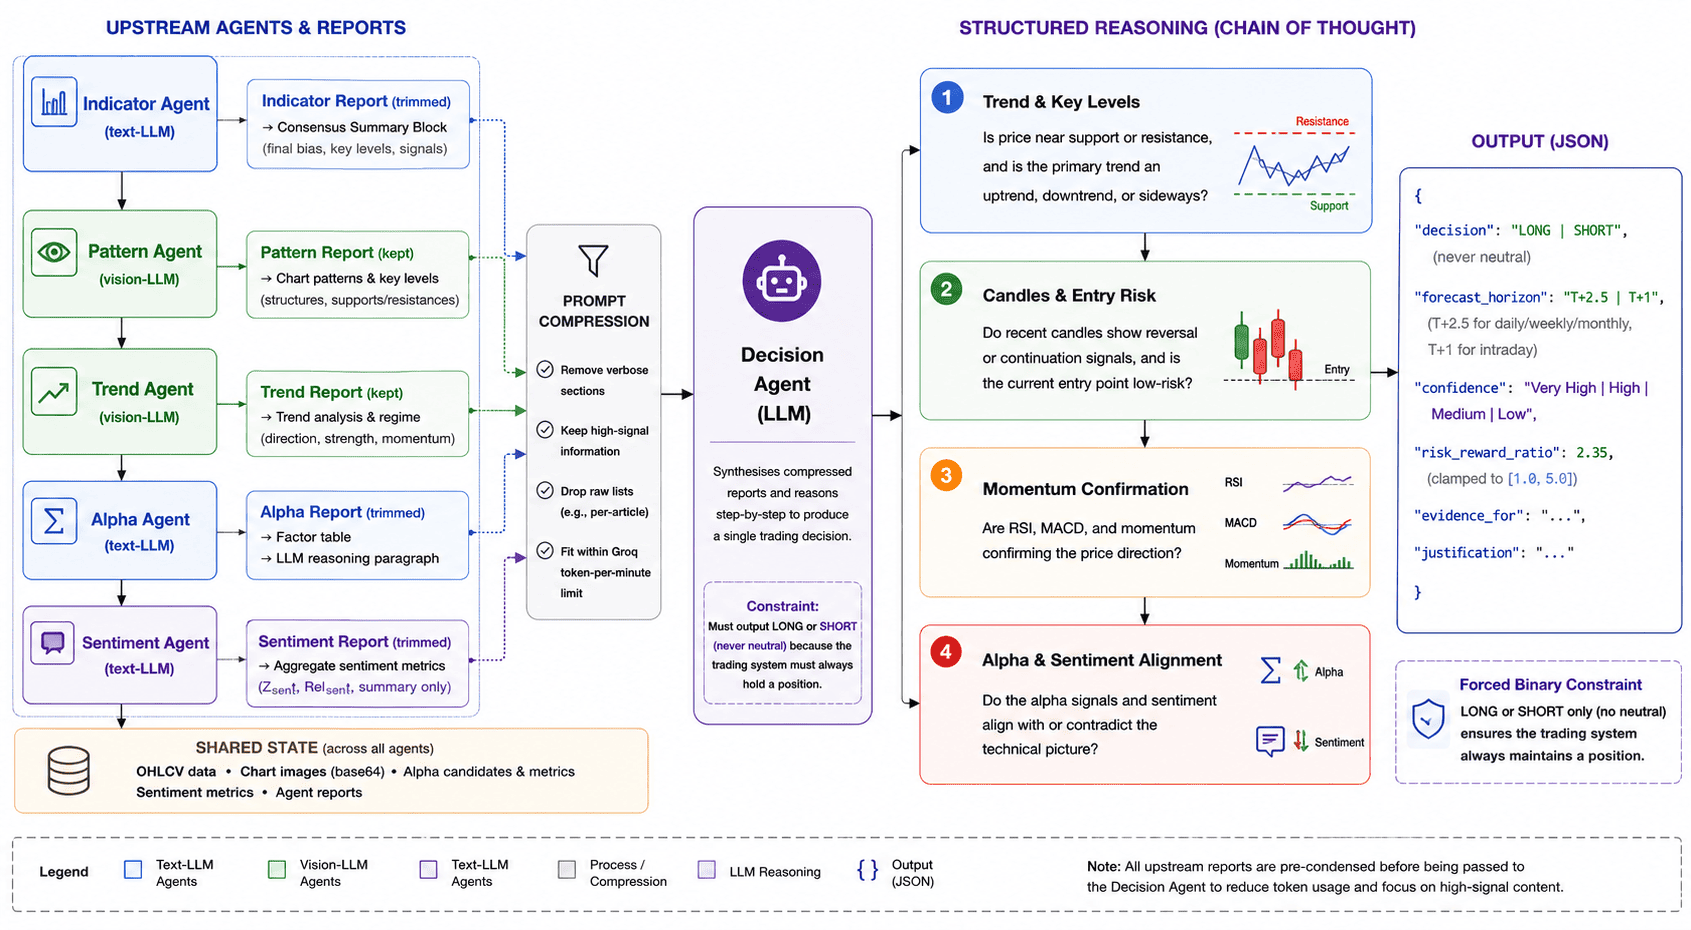
\includegraphics[width=0.95\textwidth]{figs/decision_agent_pipeline.png}
    \caption{Decision Agent reasoning pipeline}
    \label{fig:decision_agent}
\end{figure}

The agent is prompted to reason through four sequential questions in a structured chain-of-thought process. It evaluates whether the price is near support or resistance while identifying the primary trend, checks if recent candles show reversal or continuation signals to ensure a low-risk entry, verifies whether technical oscillators like RSI and MACD confirm the price direction, and finally assesses if the quantitative alpha signals and sentiment align with or contradict the technical picture.

Following this reasoning, the model must output a JSON object comprising a forced binary direction forecast (\texttt{LONG} or \texttt{SHORT}), the \texttt{forecast\_horizon}, the \texttt{confidence} level, a \texttt{risk\_reward\_ratio} clamped to $[1.0, 5.0]$, supporting and opposing evidence, and a final \texttt{justification} paragraph. The prompt explicitly states that this label is not proof of an executed order.

The forced binary constraint supports direction classification only. Downstream account logic independently maps predictions to actions: \texttt{SHORT} maps to \texttt{CASH}, whereas \texttt{LONG} invests all available cash at the next open and closes the position at the configured target close after applying costs on both legs.
